\noindent Two test cases with two models have been studied called wPCC and Optiwise. The wPCC test case is a ship model that was designed for wind-assisted propulsion systems (WAPS) and can alter between a fully sailing mode and a fully motoring mode, and in between. 
However, this study only considers the motor mode. The wPCC design differs from conventional motoring cargo ship designs in that the ship has two very large rudders, which are two to three times larger in size than needed for a conventional ship. The ship also has fins on the bilge to generate extra lift while sailing, as shown in the scale model in \autoref{fig:wPCC}.
\autoref{tab:main_particulars} shows the main particulars of the scale model. 

\begin{figure}[h]
    \centering
    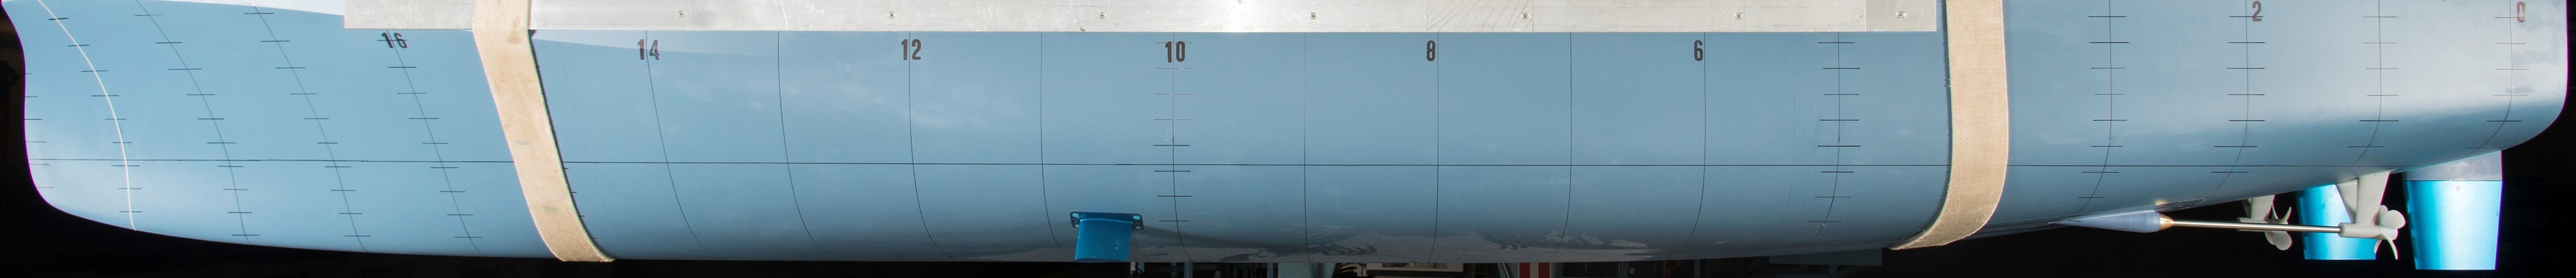
\includegraphics[width=\columnwidth]{figures/5m2.jpg}
    \caption{Scale model of the wPCC used in the model tests. Copyright RISE.}
    \label{fig:wPCC}
\end{figure}

The Optiwise test case is an ordinary VLCC tanker but with a larger rudder size than for a motoring operation mode, adopted for WAPS as shown in the scale model in \autoref{fig:optiwise} with main particulars according to \autoref{tab:main_particulars}.
Optiwise FRMTs were conducted as a continuation of the wPCC experiments, with a more conventional ship design. The experiments were run at a lower Froude number compared to the wPCC, so that wave generation and roll would have lesser impact. The larger rudder was expected to play a more important role in total hydrodynamics, compared to conventional ships. The model was therefore equipped with rudder force transducers, so that the rudder forces could be monitored during the maneuvers. 
\begin{figure}[h]
    \centering
    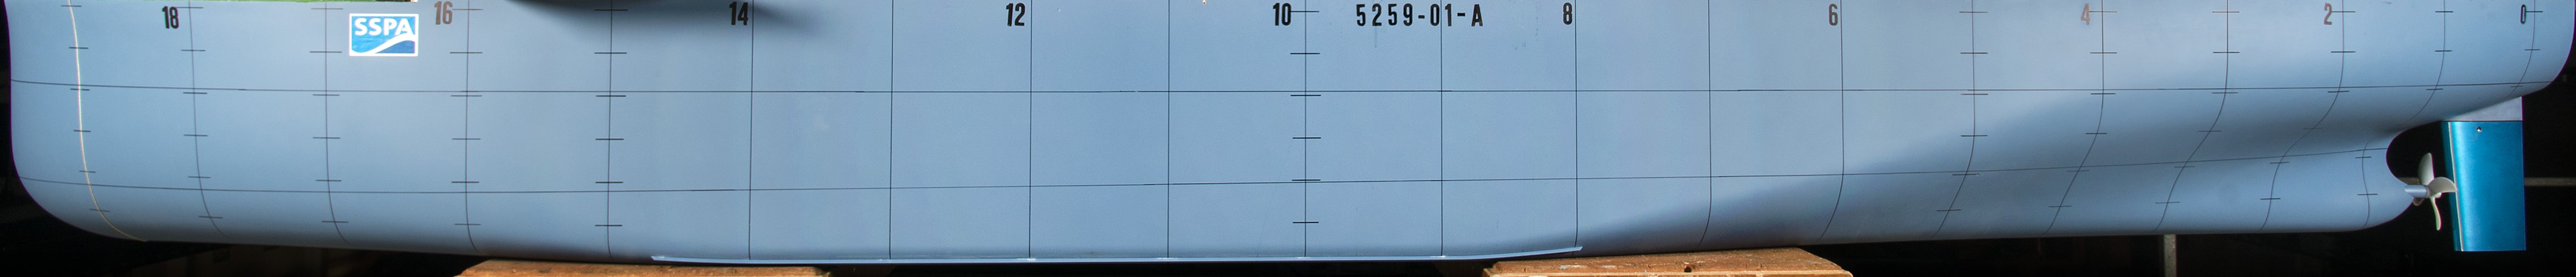
\includegraphics[width=\columnwidth]{figures/optiwise.jpg}
    \caption{Scale model of the Optiwise used in the model tests. Copyright RISE.}
    \label{fig:optiwise}
\end{figure}
\begin{table}[h]
    \centering
    \scriptsize
    \caption{Main particulars (SI units) of the wPCC scale model.}
    \label{tab:main_particulars}
    \pgfplotstabletypeset[col sep=comma, column type=r,
        columns/Parameter/.style={column type=l,string type},
        columns/Unit/.style={column type=l,string type,column name=~},
        columns/Description/.style={column type=l,string type},
        columns/Value/.style={column type=r, column name=~},
        every head row/.style={before row=\hline,after row=\hline},
        every last row/.style={after row=\hline}
    ]{tables/test_cases.main_particulars.csv}
\end{table}